% Options for packages loaded elsewhere
\PassOptionsToPackage{unicode}{hyperref}
\PassOptionsToPackage{hyphens}{url}
%
\documentclass[
]{article}
\usepackage{amsmath,amssymb}
\usepackage{lmodern}
\usepackage{ifxetex,ifluatex}
\ifnum 0\ifxetex 1\fi\ifluatex 1\fi=0 % if pdftex
  \usepackage[T1]{fontenc}
  \usepackage[utf8]{inputenc}
  \usepackage{textcomp} % provide euro and other symbols
\else % if luatex or xetex
  \usepackage{unicode-math}
  \defaultfontfeatures{Scale=MatchLowercase}
  \defaultfontfeatures[\rmfamily]{Ligatures=TeX,Scale=1}
\fi
% Use upquote if available, for straight quotes in verbatim environments
\IfFileExists{upquote.sty}{\usepackage{upquote}}{}
\IfFileExists{microtype.sty}{% use microtype if available
  \usepackage[]{microtype}
  \UseMicrotypeSet[protrusion]{basicmath} % disable protrusion for tt fonts
}{}
\makeatletter
\@ifundefined{KOMAClassName}{% if non-KOMA class
  \IfFileExists{parskip.sty}{%
    \usepackage{parskip}
  }{% else
    \setlength{\parindent}{0pt}
    \setlength{\parskip}{6pt plus 2pt minus 1pt}}
}{% if KOMA class
  \KOMAoptions{parskip=half}}
\makeatother
\usepackage{xcolor}
\IfFileExists{xurl.sty}{\usepackage{xurl}}{} % add URL line breaks if available
\IfFileExists{bookmark.sty}{\usepackage{bookmark}}{\usepackage{hyperref}}
\hypersetup{
  pdftitle={Exam 1},
  pdfauthor={Sara Whitelaw, Michaela Reiser, Rachael Villari},
  hidelinks,
  pdfcreator={LaTeX via pandoc}}
\urlstyle{same} % disable monospaced font for URLs
\usepackage[margin=1in]{geometry}
\usepackage{color}
\usepackage{fancyvrb}
\newcommand{\VerbBar}{|}
\newcommand{\VERB}{\Verb[commandchars=\\\{\}]}
\DefineVerbatimEnvironment{Highlighting}{Verbatim}{commandchars=\\\{\}}
% Add ',fontsize=\small' for more characters per line
\usepackage{framed}
\definecolor{shadecolor}{RGB}{248,248,248}
\newenvironment{Shaded}{\begin{snugshade}}{\end{snugshade}}
\newcommand{\AlertTok}[1]{\textcolor[rgb]{0.94,0.16,0.16}{#1}}
\newcommand{\AnnotationTok}[1]{\textcolor[rgb]{0.56,0.35,0.01}{\textbf{\textit{#1}}}}
\newcommand{\AttributeTok}[1]{\textcolor[rgb]{0.77,0.63,0.00}{#1}}
\newcommand{\BaseNTok}[1]{\textcolor[rgb]{0.00,0.00,0.81}{#1}}
\newcommand{\BuiltInTok}[1]{#1}
\newcommand{\CharTok}[1]{\textcolor[rgb]{0.31,0.60,0.02}{#1}}
\newcommand{\CommentTok}[1]{\textcolor[rgb]{0.56,0.35,0.01}{\textit{#1}}}
\newcommand{\CommentVarTok}[1]{\textcolor[rgb]{0.56,0.35,0.01}{\textbf{\textit{#1}}}}
\newcommand{\ConstantTok}[1]{\textcolor[rgb]{0.00,0.00,0.00}{#1}}
\newcommand{\ControlFlowTok}[1]{\textcolor[rgb]{0.13,0.29,0.53}{\textbf{#1}}}
\newcommand{\DataTypeTok}[1]{\textcolor[rgb]{0.13,0.29,0.53}{#1}}
\newcommand{\DecValTok}[1]{\textcolor[rgb]{0.00,0.00,0.81}{#1}}
\newcommand{\DocumentationTok}[1]{\textcolor[rgb]{0.56,0.35,0.01}{\textbf{\textit{#1}}}}
\newcommand{\ErrorTok}[1]{\textcolor[rgb]{0.64,0.00,0.00}{\textbf{#1}}}
\newcommand{\ExtensionTok}[1]{#1}
\newcommand{\FloatTok}[1]{\textcolor[rgb]{0.00,0.00,0.81}{#1}}
\newcommand{\FunctionTok}[1]{\textcolor[rgb]{0.00,0.00,0.00}{#1}}
\newcommand{\ImportTok}[1]{#1}
\newcommand{\InformationTok}[1]{\textcolor[rgb]{0.56,0.35,0.01}{\textbf{\textit{#1}}}}
\newcommand{\KeywordTok}[1]{\textcolor[rgb]{0.13,0.29,0.53}{\textbf{#1}}}
\newcommand{\NormalTok}[1]{#1}
\newcommand{\OperatorTok}[1]{\textcolor[rgb]{0.81,0.36,0.00}{\textbf{#1}}}
\newcommand{\OtherTok}[1]{\textcolor[rgb]{0.56,0.35,0.01}{#1}}
\newcommand{\PreprocessorTok}[1]{\textcolor[rgb]{0.56,0.35,0.01}{\textit{#1}}}
\newcommand{\RegionMarkerTok}[1]{#1}
\newcommand{\SpecialCharTok}[1]{\textcolor[rgb]{0.00,0.00,0.00}{#1}}
\newcommand{\SpecialStringTok}[1]{\textcolor[rgb]{0.31,0.60,0.02}{#1}}
\newcommand{\StringTok}[1]{\textcolor[rgb]{0.31,0.60,0.02}{#1}}
\newcommand{\VariableTok}[1]{\textcolor[rgb]{0.00,0.00,0.00}{#1}}
\newcommand{\VerbatimStringTok}[1]{\textcolor[rgb]{0.31,0.60,0.02}{#1}}
\newcommand{\WarningTok}[1]{\textcolor[rgb]{0.56,0.35,0.01}{\textbf{\textit{#1}}}}
\usepackage{graphicx}
\makeatletter
\def\maxwidth{\ifdim\Gin@nat@width>\linewidth\linewidth\else\Gin@nat@width\fi}
\def\maxheight{\ifdim\Gin@nat@height>\textheight\textheight\else\Gin@nat@height\fi}
\makeatother
% Scale images if necessary, so that they will not overflow the page
% margins by default, and it is still possible to overwrite the defaults
% using explicit options in \includegraphics[width, height, ...]{}
\setkeys{Gin}{width=\maxwidth,height=\maxheight,keepaspectratio}
% Set default figure placement to htbp
\makeatletter
\def\fps@figure{htbp}
\makeatother
\setlength{\emergencystretch}{3em} % prevent overfull lines
\providecommand{\tightlist}{%
  \setlength{\itemsep}{0pt}\setlength{\parskip}{0pt}}
\setcounter{secnumdepth}{-\maxdimen} % remove section numbering
\ifluatex
  \usepackage{selnolig}  % disable illegal ligatures
\fi

\title{Exam 1}
\author{Sara Whitelaw, Michaela Reiser, Rachael Villari}
\date{12/12/2021}

\begin{document}
\maketitle

\hypertarget{crim250-final-project---crime-distributions-at-ivy-league-institutions}{%
\section{Crim250 Final Project - Crime Distributions at Ivy League
Institutions}\label{crim250-final-project---crime-distributions-at-ivy-league-institutions}}

Loading Data: Columbia, Yale, Upenn

\begin{Shaded}
\begin{Highlighting}[]
\NormalTok{dat.Columbia }\OtherTok{\textless{}{-}} \FunctionTok{read.csv}\NormalTok{(}\StringTok{\textquotesingle{}jacobdkaplan.com\_school\_count\_Columbia University in the City of New York.csv\textquotesingle{}}\NormalTok{)}
\NormalTok{dat.Upenn }\OtherTok{\textless{}{-}} \FunctionTok{read.csv}\NormalTok{(}\StringTok{\textquotesingle{}upenndata.csv\textquotesingle{}}\NormalTok{)}
\NormalTok{dat.Yale }\OtherTok{\textless{}{-}} \FunctionTok{read.csv}\NormalTok{(}\StringTok{\textquotesingle{}jacobdkaplan.com\_school\_count\_Yale University.csv\textquotesingle{}}\NormalTok{)}
\end{Highlighting}
\end{Shaded}

\hypertarget{introduction}{%
\section{1. INTRODUCTION}\label{introduction}}

At the University level, it is important that crime trends are observed
in relation to the external factors that may have an effect. Ivy League
universities, being private institutions that receive billions of
dollars in endowments, should have ample measures in place to control
crime rates on campus to maintain the safety of students. In this
report, we will observe the total crime trends between the University of
Pennsylvania, Yale University, and Columbia University and then take a
more specific look at sexual offense trends. These trends will be
compared with external research that analyzes police funding and the
implementation of Title IX. Ultimately, it is important that more causal
research is conducted in this area to observe whether it is beneficial
to have privately funded university police departments and whether to
bolster Title IX power. The data used in this report contain the total
crime data from 2001-2017 for the three Ivy League institutions
mentioned above.

\hypertarget{exploratory-data-analysis}{%
\section{2. EXPLORATORY DATA ANALYSIS}\label{exploratory-data-analysis}}

\hypertarget{data-description}{%
\paragraph{2.1 Data Description}\label{data-description}}

The selected dataset was compiled data from Jacob Kaplan on total crimes
reported at Universities.1 All of the data comes from the Department of
Education Office of Postsecondary Education, which collects crime data
from colleges. The following variables were the focus of the analysis:
total number of aggravated assault, total number of arson, total number
of motor vehicle theft, total number of non-negligent manslaughter,
total number of negligent manslaughter, total number of sex offenses.
The variables total number of on campus sex crimes and total number of
off campus sex crimes were explored as well. All datasets used for this
analysis individually contain 17 years of data with 1039 observations.

\begin{Shaded}
\begin{Highlighting}[]
\FunctionTok{dim}\NormalTok{(dat.Columbia)}
\end{Highlighting}
\end{Shaded}

\begin{verbatim}
## [1]   17 1039
\end{verbatim}

\begin{Shaded}
\begin{Highlighting}[]
\FunctionTok{dim}\NormalTok{(dat.Yale)}
\end{Highlighting}
\end{Shaded}

\begin{verbatim}
## [1]   17 1039
\end{verbatim}

\begin{Shaded}
\begin{Highlighting}[]
\FunctionTok{dim}\NormalTok{(dat.Upenn)}
\end{Highlighting}
\end{Shaded}

\begin{verbatim}
## [1]   17 1039
\end{verbatim}

\hypertarget{missing-values}{%
\paragraph{2.2 MISSING VALUES}\label{missing-values}}

There are many missing values because, different from the value of 0,
there are crime ``categories'' that do not have any reported crime data
for certain years. For example, looking at the University of
Pennsylvania data, there is no data for off-campus rape crimes until
2014. This will affect our data analysis, because the crime statistics
may seem lower than they actually are.

\hypertarget{university-locations}{%
\paragraph{2.3 UNIVERSITY LOCATIONS}\label{university-locations}}

The three universities are located in urban settings. University of
Pennsylvania is located in Philadelphia, PA (2019 pop. = 1.58 million).2
Columbia University is located in New York City, NY (2019 pop. = 8.33
million).2 Yale University is in New Haven, CT (2019 pop. = 130,250).2
All population data was retrieved from the US census population
estimates.

\hypertarget{campus-police-force}{%
\paragraph{2.4 CAMPUS POLICE FORCE}\label{campus-police-force}}

\begin{verbatim}
The University of Pennsylvania’s Division of Public Safety (DPS) comprises 180 personnel and 121 of these are sworn-in University of Pennsylvania police officers.3 The Yale Police Department (YPD) comprises 93 sworn-in police officers.4 Due to New York regulations, Columbia University has 147 full-time security officers and no sworn-in officers.5  These security officers cannot carry firearms or arrest individuals, but they can detain suspected criminals on the University property. However, Columbia University is in the 26th precinct of the NYPD.6 
\end{verbatim}

\hypertarget{total-crimes-per-year}{%
\paragraph{2.5 TOTAL CRIMES PER YEAR}\label{total-crimes-per-year}}

\begin{Shaded}
\begin{Highlighting}[]
\FunctionTok{plot}\NormalTok{(dat.Columbia}\SpecialCharTok{$}\NormalTok{year, dat.Columbia}\SpecialCharTok{$}\NormalTok{crimes\_total\_total, }\AttributeTok{type =} \StringTok{"b"}\NormalTok{, }\AttributeTok{main =} \StringTok{"Scatterplot of Total Number of Reported Crimes at Columbia from 2001{-}2017"}\NormalTok{,}
     \AttributeTok{xlab =} \StringTok{"Year"}\NormalTok{, }\AttributeTok{ylab =} \StringTok{"Number of offenses reported to police"}\NormalTok{, }\AttributeTok{cex.axis =} \FloatTok{0.75}\NormalTok{)}

\FunctionTok{axis}\NormalTok{(}\DecValTok{1}\NormalTok{, }\AttributeTok{at=}\FunctionTok{seq}\NormalTok{(}\DecValTok{2001}\NormalTok{,}\DecValTok{2017}\NormalTok{,}\DecValTok{1}\NormalTok{), }\AttributeTok{cex.axis=}\FloatTok{0.75}\NormalTok{)}
\end{Highlighting}
\end{Shaded}

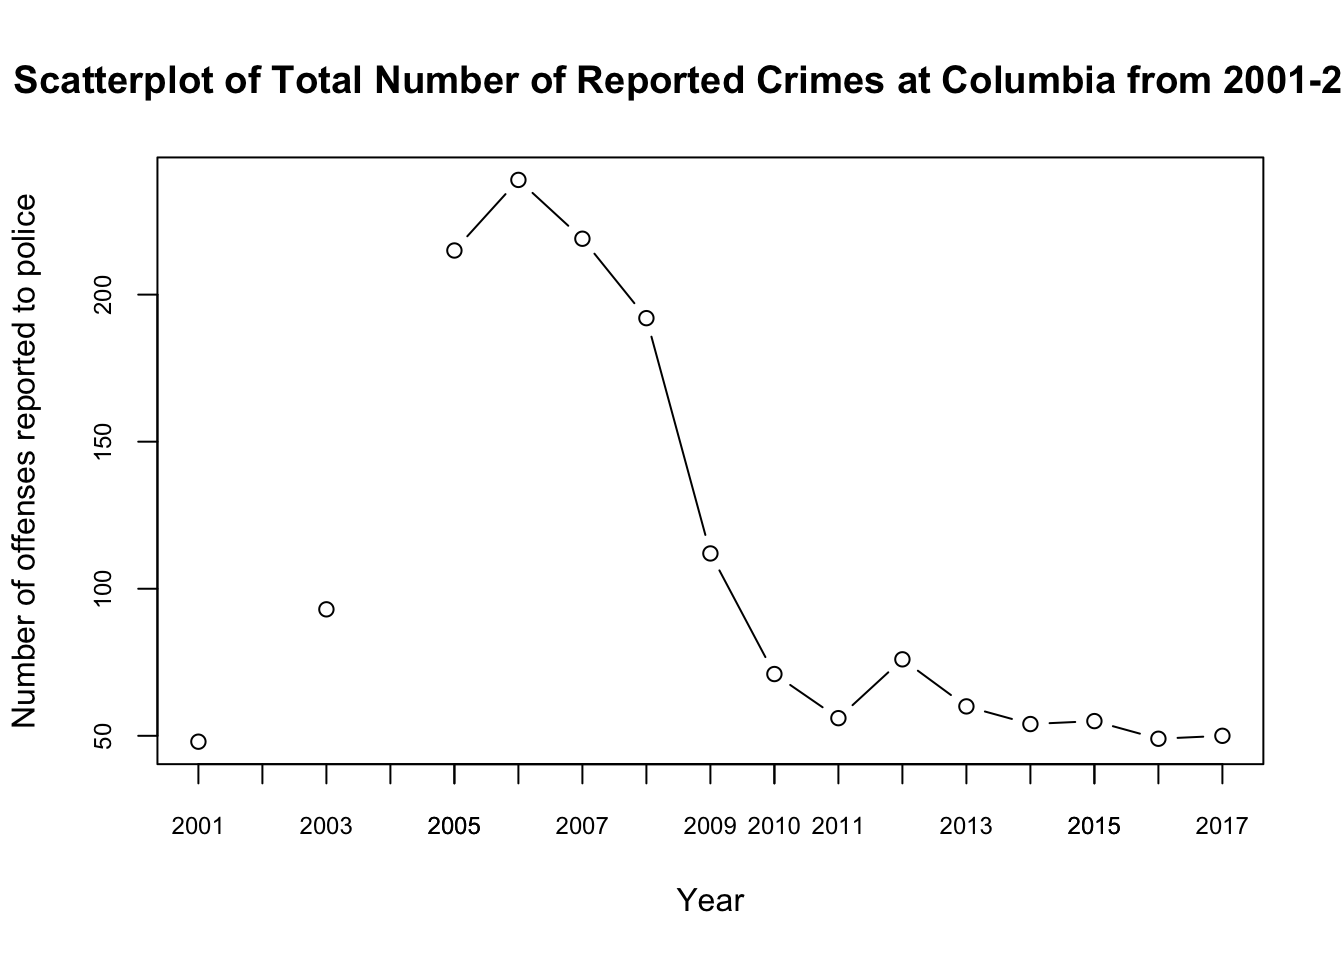
\includegraphics{Crim250FinalProj_files/figure-latex/unnamed-chunk-3-1.pdf}

\begin{Shaded}
\begin{Highlighting}[]
\FunctionTok{plot}\NormalTok{(dat.Yale}\SpecialCharTok{$}\NormalTok{year, dat.Yale}\SpecialCharTok{$}\NormalTok{crimes\_total\_total, }\AttributeTok{type =} \StringTok{"b"}\NormalTok{, }\AttributeTok{main =} \StringTok{"Scatterplot of Total Number of Reported Crimes at Yale from 2001{-}2017"}\NormalTok{,}
     \AttributeTok{xlab =} \StringTok{"Year"}\NormalTok{, }\AttributeTok{ylab =} \StringTok{"Number of offenses reported to police"}\NormalTok{, }\AttributeTok{cex.axis =} \FloatTok{0.75}\NormalTok{)}

\FunctionTok{axis}\NormalTok{(}\DecValTok{1}\NormalTok{, }\AttributeTok{at=}\FunctionTok{seq}\NormalTok{(}\DecValTok{2001}\NormalTok{,}\DecValTok{2017}\NormalTok{,}\DecValTok{1}\NormalTok{), }\AttributeTok{cex.axis=}\FloatTok{0.75}\NormalTok{)}
\end{Highlighting}
\end{Shaded}

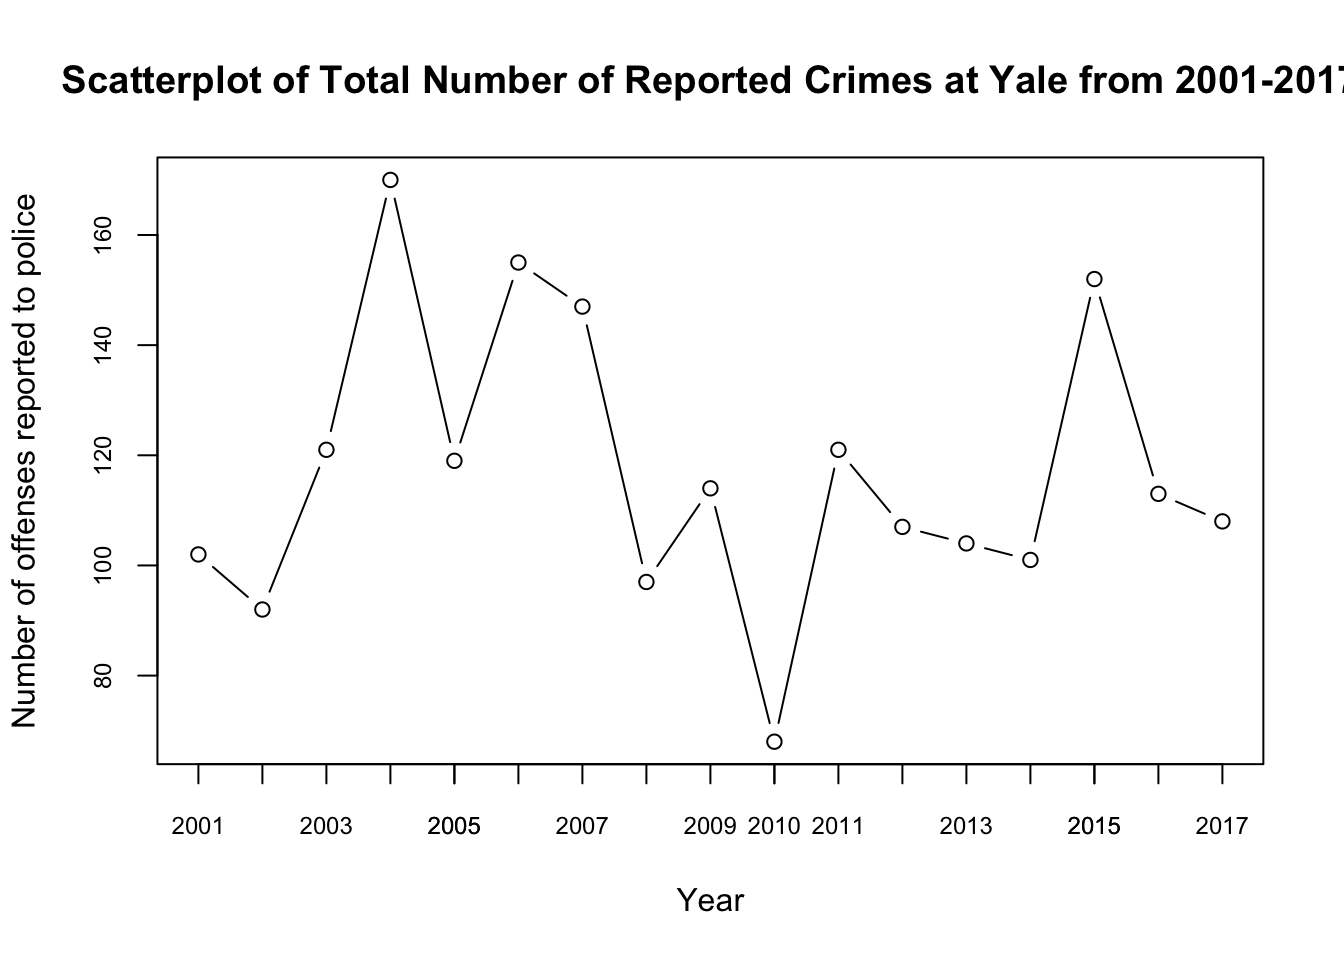
\includegraphics{Crim250FinalProj_files/figure-latex/unnamed-chunk-3-2.pdf}

\begin{Shaded}
\begin{Highlighting}[]
\FunctionTok{plot}\NormalTok{(dat.Upenn}\SpecialCharTok{$}\NormalTok{year, dat.Upenn}\SpecialCharTok{$}\NormalTok{crimes\_total\_total, }\AttributeTok{type =} \StringTok{"b"}\NormalTok{, }\AttributeTok{main =} \StringTok{"Scatterplot of Total Number of Reported Crimes at UPenn from 2001{-}2017"}\NormalTok{,}
     \AttributeTok{xlab =} \StringTok{"Year"}\NormalTok{, }\AttributeTok{ylab =} \StringTok{"Number of offenses reported to police"}\NormalTok{, }\AttributeTok{cex.axis =} \FloatTok{0.75}\NormalTok{)}

\FunctionTok{axis}\NormalTok{(}\DecValTok{1}\NormalTok{, }\AttributeTok{at=}\FunctionTok{seq}\NormalTok{(}\DecValTok{2001}\NormalTok{,}\DecValTok{2017}\NormalTok{,}\DecValTok{1}\NormalTok{), }\AttributeTok{cex.axis=}\FloatTok{0.75}\NormalTok{)}
\end{Highlighting}
\end{Shaded}

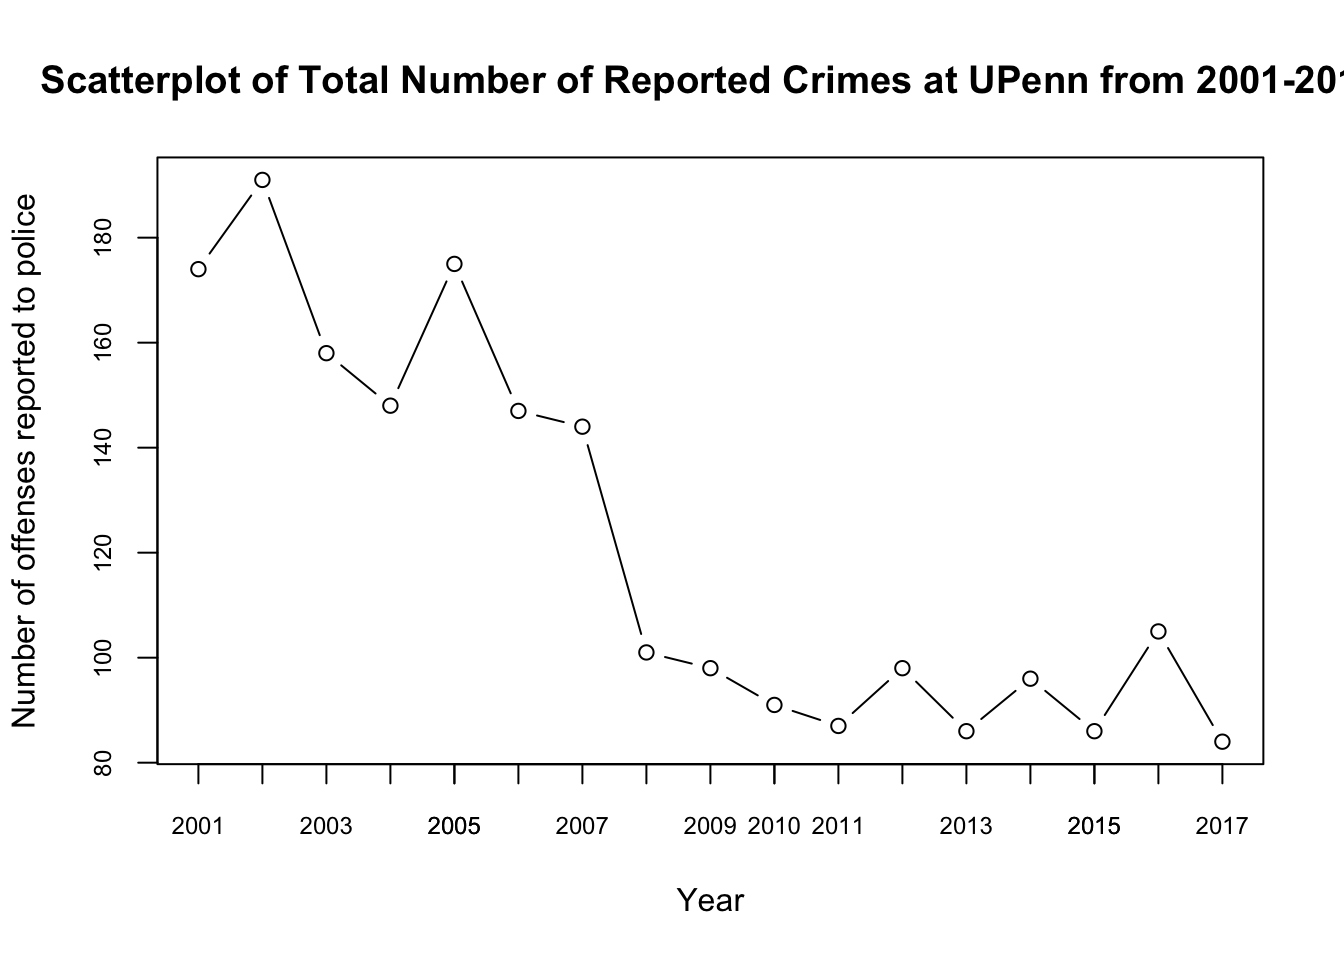
\includegraphics{Crim250FinalProj_files/figure-latex/unnamed-chunk-3-3.pdf}

\hypertarget{average-of-total-sex-offenses-per-year}{%
\paragraph{2.6 AVERAGE OF TOTAL SEX OFFENSES PER
YEAR}\label{average-of-total-sex-offenses-per-year}}

\begin{Shaded}
\begin{Highlighting}[]
\FunctionTok{plot}\NormalTok{(dat.Columbia}\SpecialCharTok{$}\NormalTok{year, dat.Columbia}\SpecialCharTok{$}\NormalTok{crimes\_total\_sex\_offenses\_total,  }\AttributeTok{type =} \StringTok{"b"}\NormalTok{, }\AttributeTok{main =} \StringTok{"Scatterplot of Total Number of Reported Sex Crimes at Columbia from 2001{-}2017"}\NormalTok{,}
     \AttributeTok{xlab =} \StringTok{"Year"}\NormalTok{, }\AttributeTok{ylab =} \StringTok{"Number of Offenses Reported to Police"}\NormalTok{, }\AttributeTok{cex.axis =} \FloatTok{0.75}\NormalTok{)}

\FunctionTok{axis}\NormalTok{(}\DecValTok{1}\NormalTok{, }\AttributeTok{at=}\FunctionTok{seq}\NormalTok{(}\DecValTok{2001}\NormalTok{,}\DecValTok{2017}\NormalTok{,}\DecValTok{1}\NormalTok{), }\AttributeTok{cex.axis=}\FloatTok{0.75}\NormalTok{)}
\end{Highlighting}
\end{Shaded}

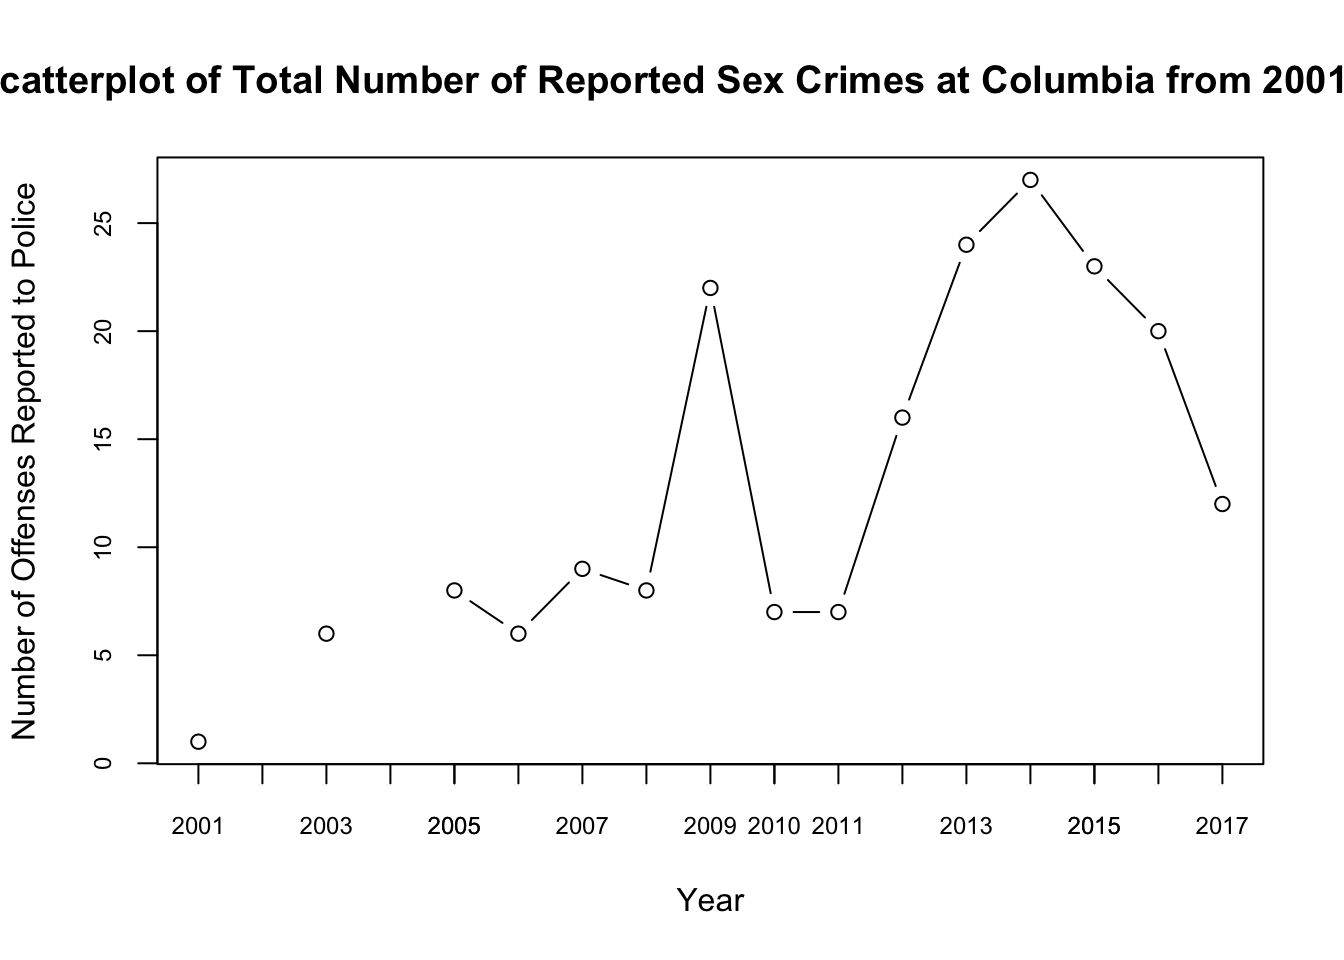
\includegraphics{Crim250FinalProj_files/figure-latex/unnamed-chunk-4-1.pdf}

\begin{Shaded}
\begin{Highlighting}[]
\FunctionTok{plot}\NormalTok{(dat.Yale}\SpecialCharTok{$}\NormalTok{year, dat.Yale}\SpecialCharTok{$}\NormalTok{crimes\_total\_sex\_offenses\_total,  }\AttributeTok{type =} \StringTok{"b"}\NormalTok{, }\AttributeTok{main =} \StringTok{"Scatterplot of Total Number of Reported Sex Crimes at Yale from 2001{-}2017"}\NormalTok{,}
     \AttributeTok{xlab =} \StringTok{"Year"}\NormalTok{, }\AttributeTok{ylab =} \StringTok{"Number of Offenses Reported to Police"}\NormalTok{, }\AttributeTok{cex.axis =} \FloatTok{0.75}\NormalTok{)}

\FunctionTok{axis}\NormalTok{(}\DecValTok{1}\NormalTok{, }\AttributeTok{at=}\FunctionTok{seq}\NormalTok{(}\DecValTok{2001}\NormalTok{,}\DecValTok{2017}\NormalTok{,}\DecValTok{1}\NormalTok{), }\AttributeTok{cex.axis=}\FloatTok{0.75}\NormalTok{)}
\end{Highlighting}
\end{Shaded}

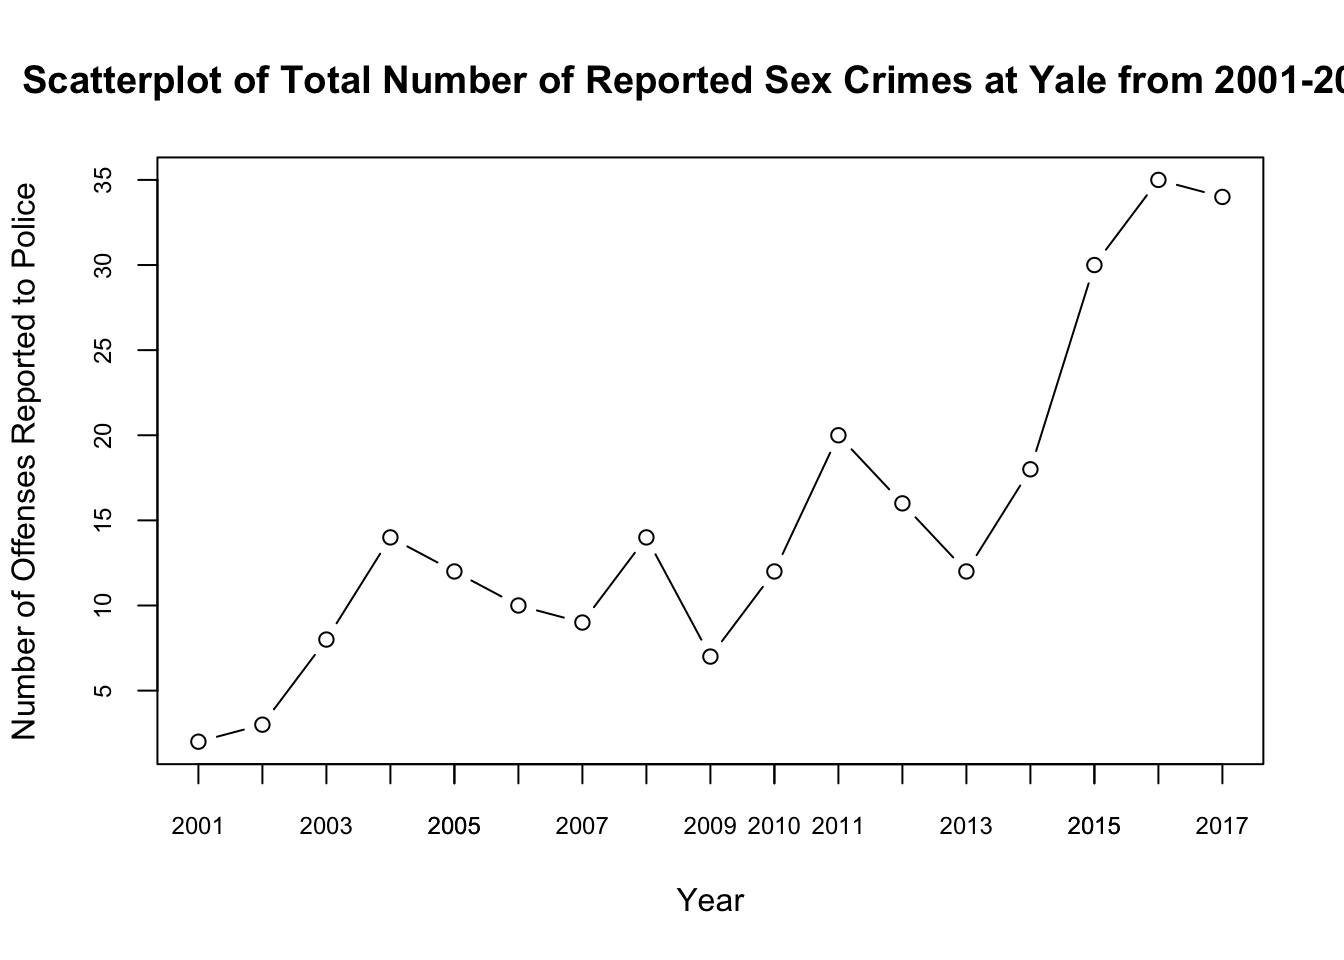
\includegraphics{Crim250FinalProj_files/figure-latex/unnamed-chunk-4-2.pdf}

\begin{Shaded}
\begin{Highlighting}[]
\FunctionTok{plot}\NormalTok{(dat.Upenn}\SpecialCharTok{$}\NormalTok{year, dat.Upenn}\SpecialCharTok{$}\NormalTok{crimes\_total\_sex\_offenses\_total,  }\AttributeTok{type =} \StringTok{"b"}\NormalTok{, }\AttributeTok{main =} \StringTok{"Scatterplot of Total Number of Reported Sex Crimes at Upenn from 2001{-}2017"}\NormalTok{,}
     \AttributeTok{xlab =} \StringTok{"Year"}\NormalTok{, }\AttributeTok{ylab =} \StringTok{"Number of Offenses Reported to Police"}\NormalTok{, }\AttributeTok{cex.axis =} \FloatTok{0.75}\NormalTok{)}

\FunctionTok{axis}\NormalTok{(}\DecValTok{1}\NormalTok{, }\AttributeTok{at=}\FunctionTok{seq}\NormalTok{(}\DecValTok{2001}\NormalTok{,}\DecValTok{2017}\NormalTok{,}\DecValTok{1}\NormalTok{), }\AttributeTok{cex.axis=}\FloatTok{0.75}\NormalTok{)}
\end{Highlighting}
\end{Shaded}

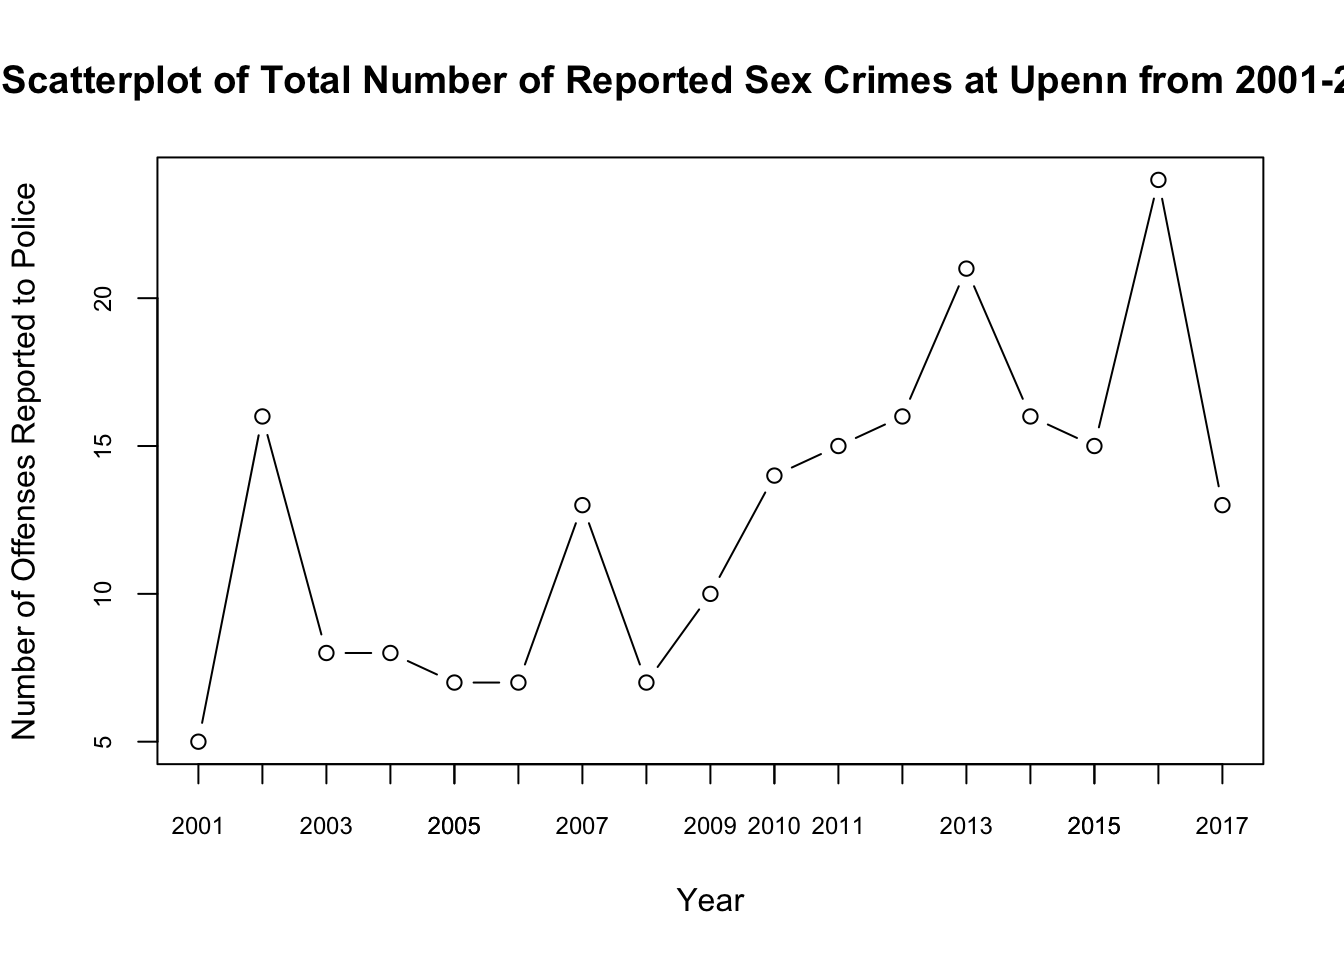
\includegraphics{Crim250FinalProj_files/figure-latex/unnamed-chunk-4-3.pdf}

\hypertarget{differences-by-onoff-campus}{%
\paragraph{2.7 DIFFERENCES BY ON/OFF
CAMPUS}\label{differences-by-onoff-campus}}

\hypertarget{on-campus-sex-offenses}{%
\paragraph{2.7.1 ON CAMPUS SEX OFFENSES}\label{on-campus-sex-offenses}}

\begin{Shaded}
\begin{Highlighting}[]
\FunctionTok{plot}\NormalTok{(dat.Columbia}\SpecialCharTok{$}\NormalTok{year, dat.Columbia}\SpecialCharTok{$}\NormalTok{crimes\_on\_campus\_sex\_offenses\_total,  }\AttributeTok{type =} \StringTok{"b"}\NormalTok{, }\AttributeTok{main =} \StringTok{"Scatterplot of On Campus Total Number of Reported Sex Crimes at Columbia from 2001{-}2017"}\NormalTok{,}
     \AttributeTok{xlab =} \StringTok{"Year"}\NormalTok{, }\AttributeTok{ylab =} \StringTok{"Number of Offenses Reported to Police"}\NormalTok{, }\AttributeTok{cex.axis =} \FloatTok{0.75}\NormalTok{)}

\FunctionTok{axis}\NormalTok{(}\DecValTok{1}\NormalTok{, }\AttributeTok{at=}\FunctionTok{seq}\NormalTok{(}\DecValTok{2001}\NormalTok{,}\DecValTok{2017}\NormalTok{,}\DecValTok{1}\NormalTok{), }\AttributeTok{cex.axis=}\FloatTok{0.75}\NormalTok{)}
\end{Highlighting}
\end{Shaded}

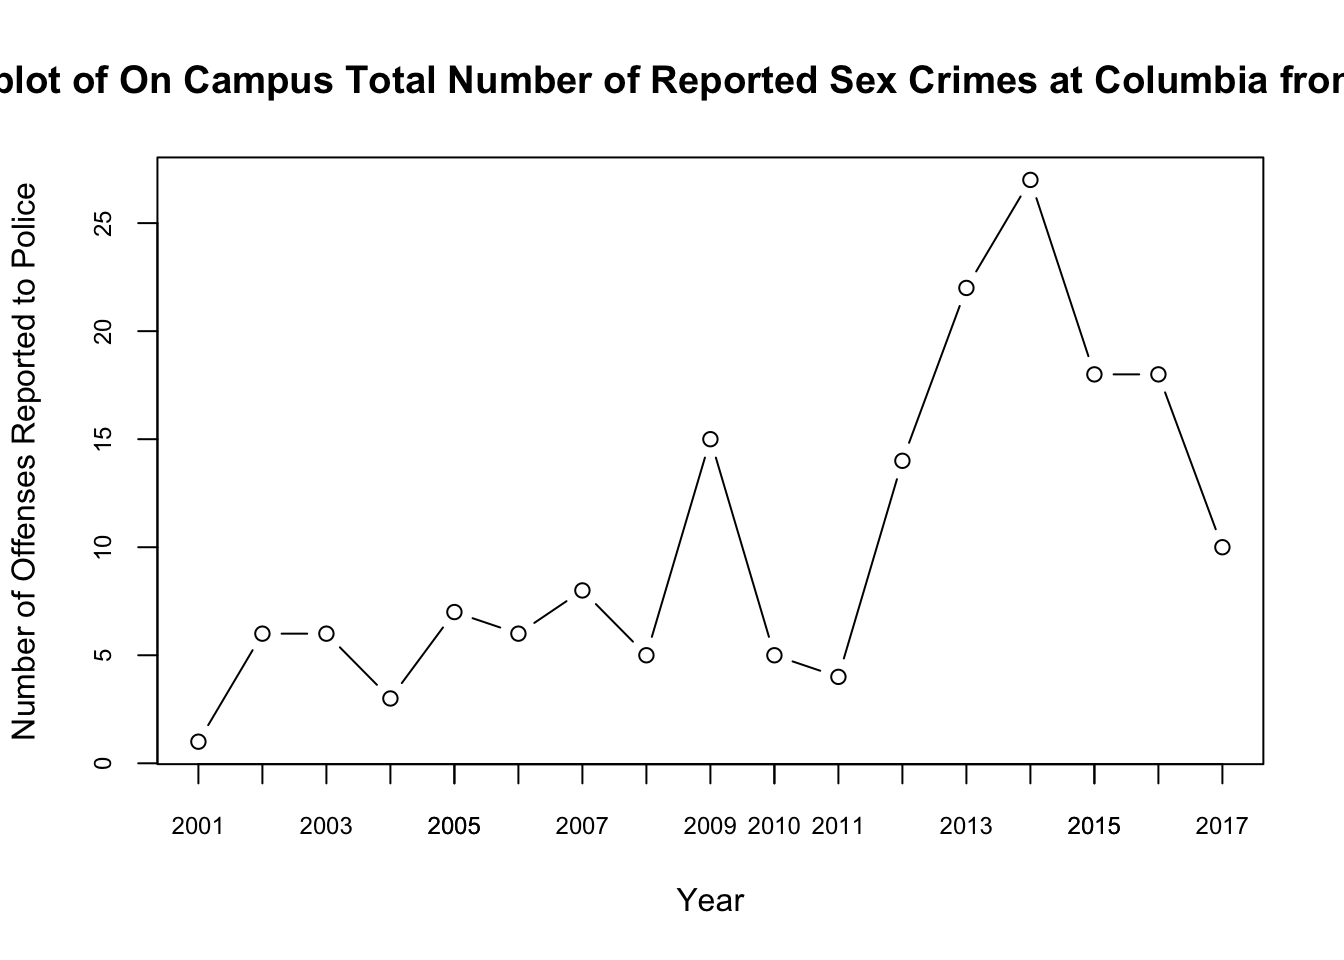
\includegraphics{Crim250FinalProj_files/figure-latex/unnamed-chunk-5-1.pdf}

\begin{Shaded}
\begin{Highlighting}[]
\FunctionTok{plot}\NormalTok{(dat.Yale}\SpecialCharTok{$}\NormalTok{year, dat.Yale}\SpecialCharTok{$}\NormalTok{crimes\_on\_campus\_sex\_offenses\_total,  }\AttributeTok{type =} \StringTok{"b"}\NormalTok{, }\AttributeTok{main =} \StringTok{"Scatterplot of On Campus Total Number of Reported Sex Crimes at Yale from 2001{-}2017"}\NormalTok{,}
     \AttributeTok{xlab =} \StringTok{"Year"}\NormalTok{, }\AttributeTok{ylab =} \StringTok{"Number of Offenses Reported to Police"}\NormalTok{, }\AttributeTok{cex.axis =} \FloatTok{0.75}\NormalTok{)}

\FunctionTok{axis}\NormalTok{(}\DecValTok{1}\NormalTok{, }\AttributeTok{at=}\FunctionTok{seq}\NormalTok{(}\DecValTok{2001}\NormalTok{,}\DecValTok{2017}\NormalTok{,}\DecValTok{1}\NormalTok{), }\AttributeTok{cex.axis=}\FloatTok{0.75}\NormalTok{)}
\end{Highlighting}
\end{Shaded}

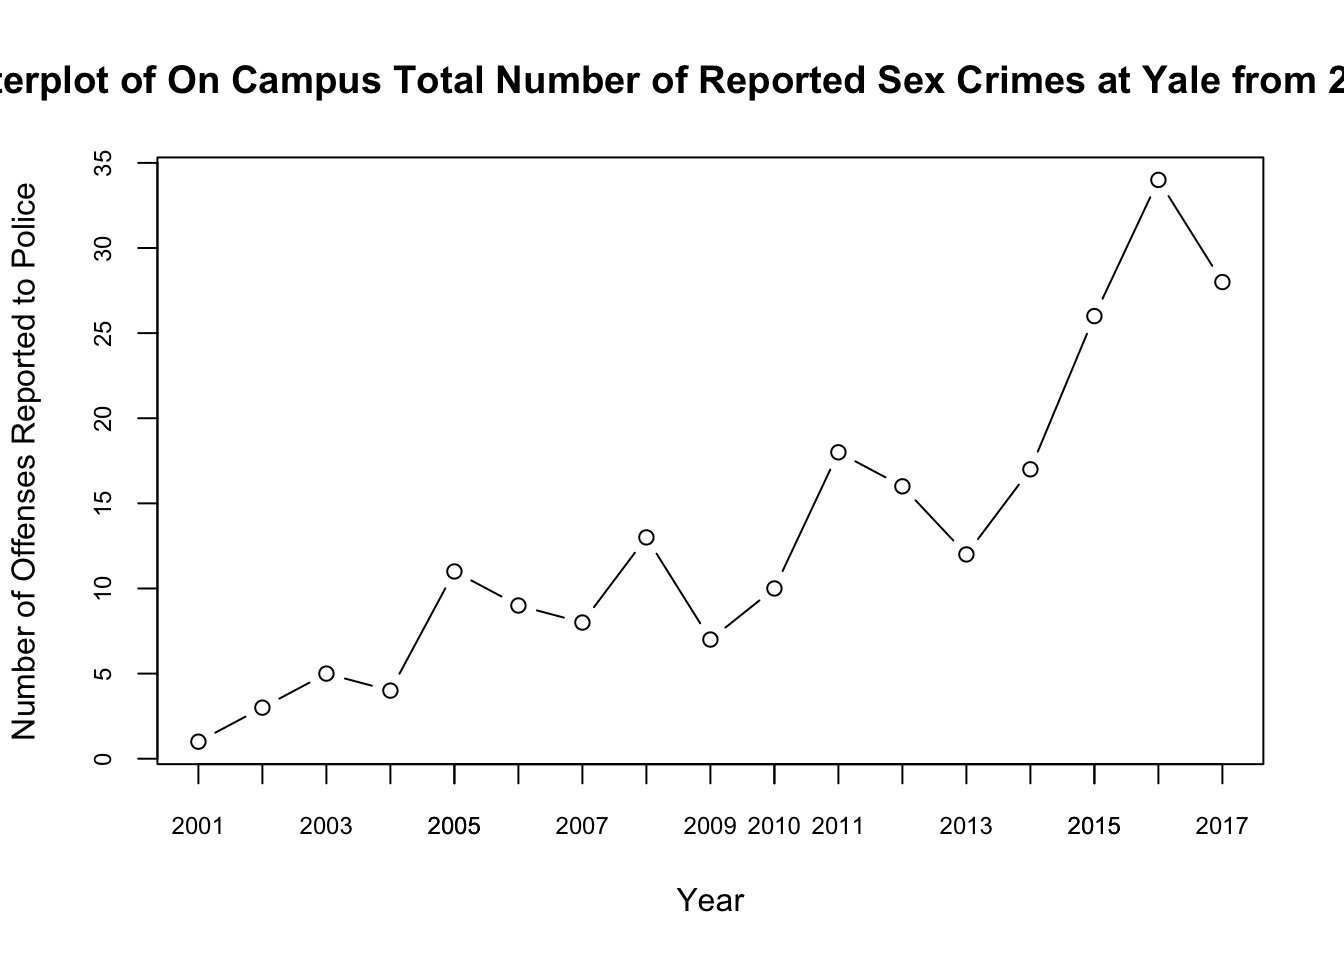
\includegraphics{Crim250FinalProj_files/figure-latex/unnamed-chunk-5-2.pdf}

\begin{Shaded}
\begin{Highlighting}[]
\FunctionTok{plot}\NormalTok{(dat.Upenn}\SpecialCharTok{$}\NormalTok{year, dat.Upenn}\SpecialCharTok{$}\NormalTok{crimes\_on\_campus\_sex\_offenses\_total,  }\AttributeTok{type =} \StringTok{"b"}\NormalTok{, }\AttributeTok{main =} \StringTok{"Scatterplot of On Campus Total Number of Reported Sex Crimes at UPenn from 2001{-}2017"}\NormalTok{,}
     \AttributeTok{xlab =} \StringTok{"Year"}\NormalTok{, }\AttributeTok{ylab =} \StringTok{"Number of Offenses Reported to Police"}\NormalTok{, }\AttributeTok{cex.axis =} \FloatTok{0.75}\NormalTok{)}

\FunctionTok{axis}\NormalTok{(}\DecValTok{1}\NormalTok{, }\AttributeTok{at=}\FunctionTok{seq}\NormalTok{(}\DecValTok{2001}\NormalTok{,}\DecValTok{2017}\NormalTok{,}\DecValTok{1}\NormalTok{), }\AttributeTok{cex.axis=}\FloatTok{0.75}\NormalTok{)}
\end{Highlighting}
\end{Shaded}

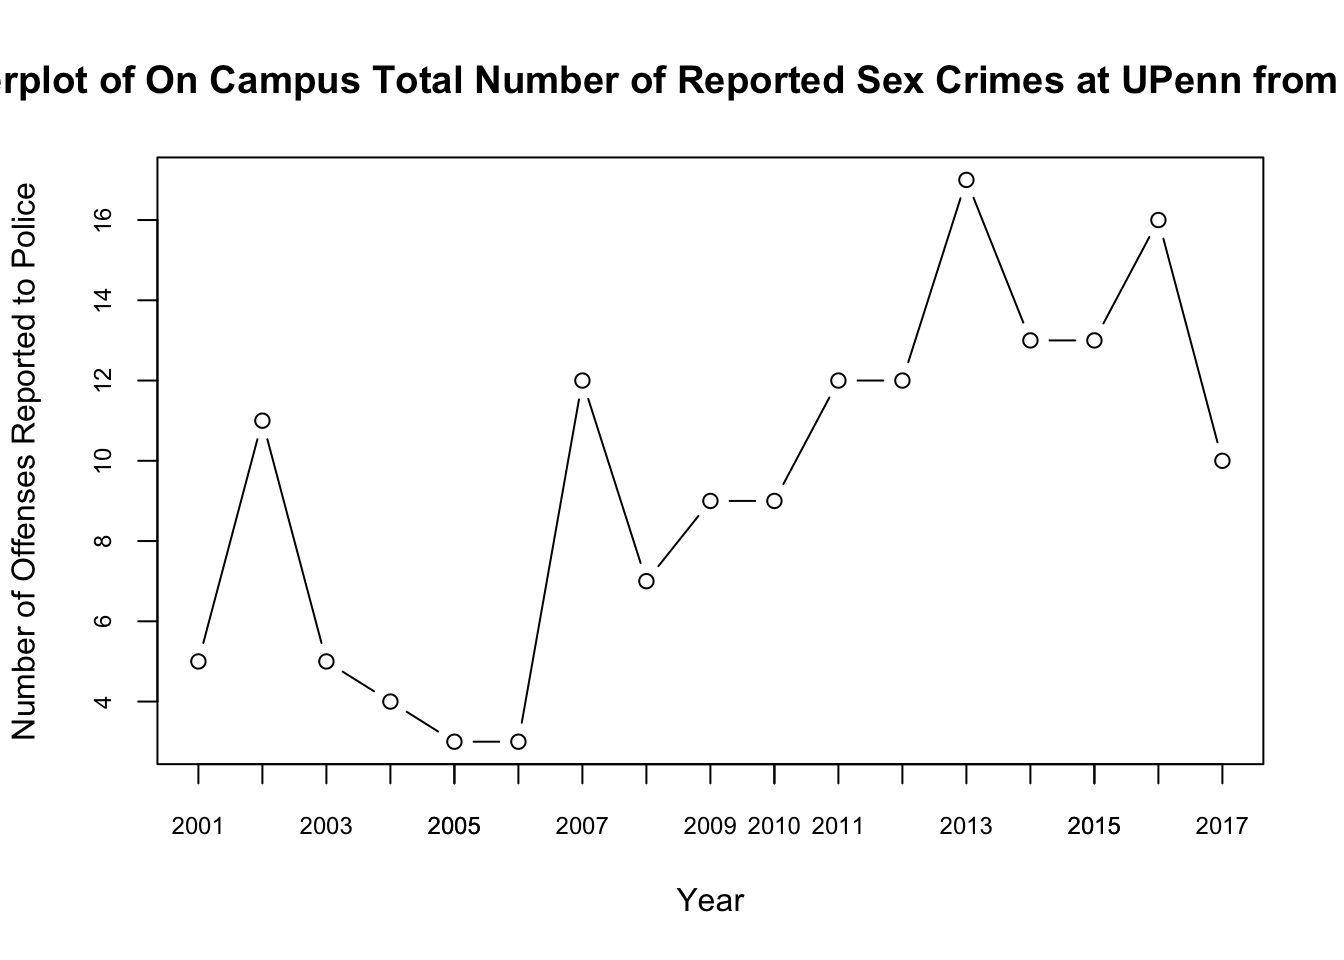
\includegraphics{Crim250FinalProj_files/figure-latex/unnamed-chunk-5-3.pdf}

2.7.2 OFF CAMPUS SEX OFFENSES

\begin{Shaded}
\begin{Highlighting}[]
\FunctionTok{plot}\NormalTok{(dat.Columbia}\SpecialCharTok{$}\NormalTok{year, dat.Columbia}\SpecialCharTok{$}\NormalTok{crimes\_noncampus\_sex\_offenses\_total,  }\AttributeTok{type =} \StringTok{"b"}\NormalTok{, }\AttributeTok{main =} \StringTok{"Scatterplot of Off Campus Total Number of Reported Sex Crimes at Columbia from 2001{-}2017"}\NormalTok{,}
     \AttributeTok{xlab =} \StringTok{"Year"}\NormalTok{, }\AttributeTok{ylab =} \StringTok{"Number of Offenses Reported to Police"}\NormalTok{, }\AttributeTok{cex.axis =} \FloatTok{0.75}\NormalTok{)}

\FunctionTok{axis}\NormalTok{(}\DecValTok{1}\NormalTok{, }\AttributeTok{at=}\FunctionTok{seq}\NormalTok{(}\DecValTok{2001}\NormalTok{,}\DecValTok{2017}\NormalTok{,}\DecValTok{1}\NormalTok{), }\AttributeTok{cex.axis=}\FloatTok{0.75}\NormalTok{)}
\end{Highlighting}
\end{Shaded}

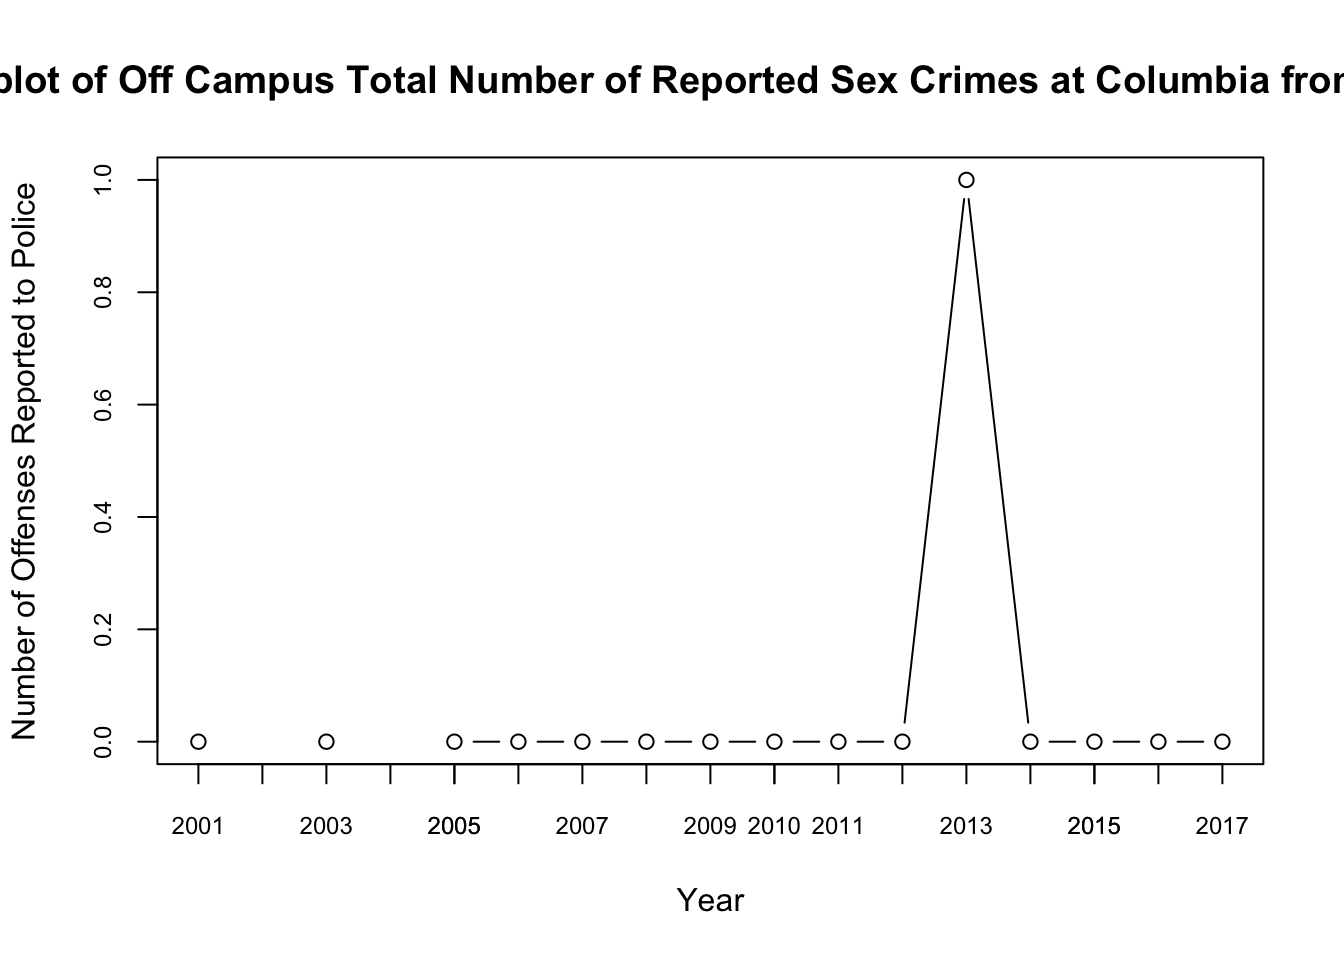
\includegraphics{Crim250FinalProj_files/figure-latex/unnamed-chunk-6-1.pdf}

\begin{Shaded}
\begin{Highlighting}[]
\FunctionTok{plot}\NormalTok{(dat.Yale}\SpecialCharTok{$}\NormalTok{year, dat.Yale}\SpecialCharTok{$}\NormalTok{crimes\_noncampus\_sex\_offenses\_total,  }\AttributeTok{type =} \StringTok{"b"}\NormalTok{, }\AttributeTok{main =} \StringTok{"Scatterplot of Off Campus Total Number of Reported Sex Crimes at Yale from 2001{-}2017"}\NormalTok{,}
     \AttributeTok{xlab =} \StringTok{"Year"}\NormalTok{, }\AttributeTok{ylab =} \StringTok{"Number of Offenses Reported to Police"}\NormalTok{, }\AttributeTok{cex.axis =} \FloatTok{0.75}\NormalTok{)}

\FunctionTok{axis}\NormalTok{(}\DecValTok{1}\NormalTok{, }\AttributeTok{at=}\FunctionTok{seq}\NormalTok{(}\DecValTok{2001}\NormalTok{,}\DecValTok{2017}\NormalTok{,}\DecValTok{1}\NormalTok{), }\AttributeTok{cex.axis=}\FloatTok{0.75}\NormalTok{)}
\end{Highlighting}
\end{Shaded}

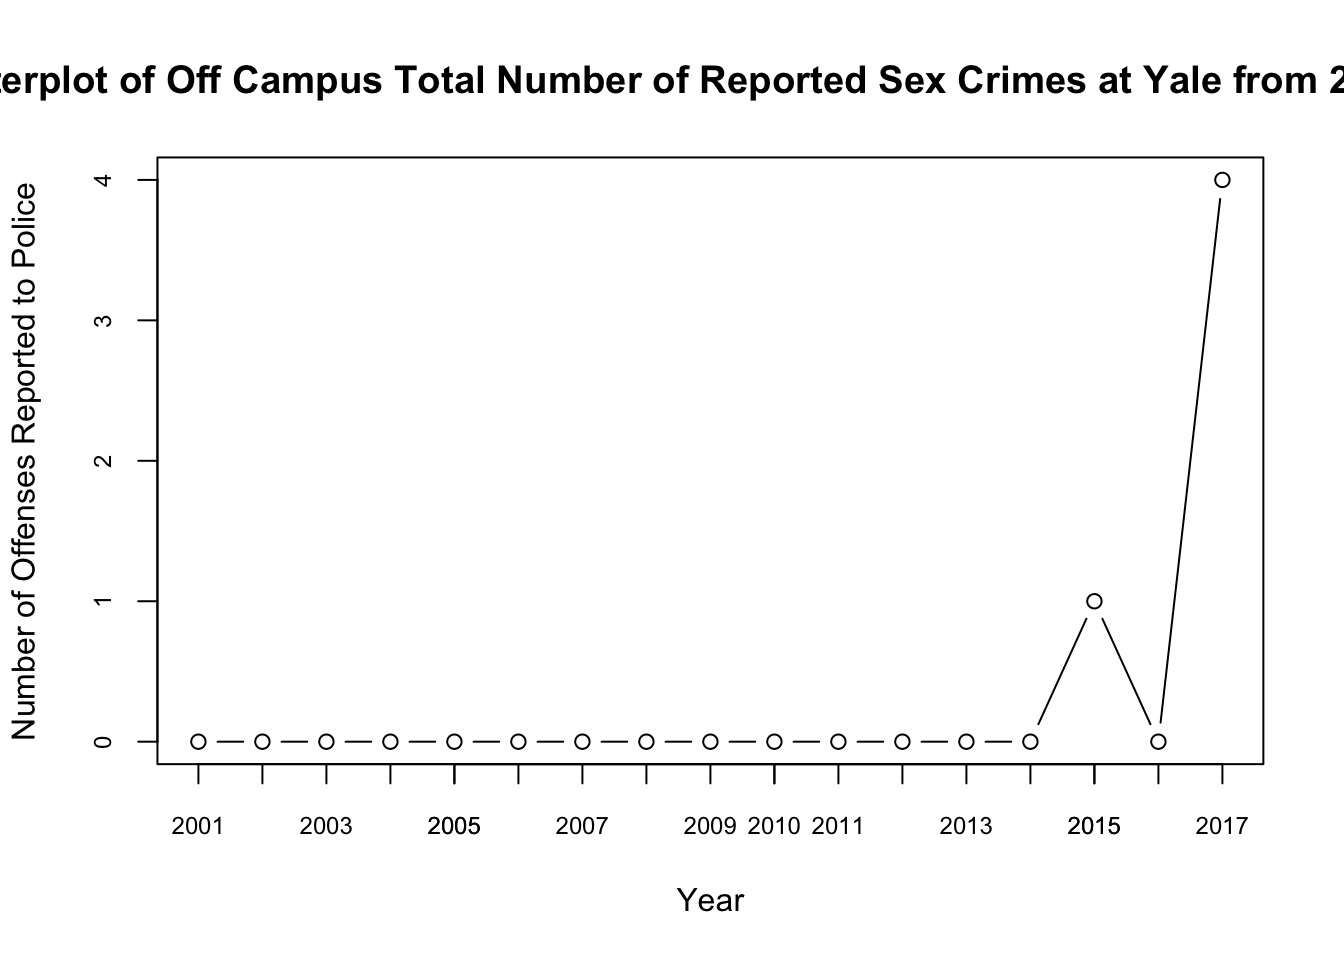
\includegraphics{Crim250FinalProj_files/figure-latex/unnamed-chunk-6-2.pdf}

\begin{Shaded}
\begin{Highlighting}[]
\FunctionTok{plot}\NormalTok{(dat.Upenn}\SpecialCharTok{$}\NormalTok{year, dat.Upenn}\SpecialCharTok{$}\NormalTok{crimes\_noncampus\_sex\_offenses\_total,  }\AttributeTok{type =} \StringTok{"b"}\NormalTok{, }\AttributeTok{main =} \StringTok{"Scatterplot of Off Campus Total Number of Reported Sex Crimes at Upenn from 2001{-}2017"}\NormalTok{,}
     \AttributeTok{xlab =} \StringTok{"Year"}\NormalTok{, }\AttributeTok{ylab =} \StringTok{"Number of Offenses Reported to Police"}\NormalTok{, }\AttributeTok{cex.axis =} \FloatTok{0.75}\NormalTok{)}

\FunctionTok{axis}\NormalTok{(}\DecValTok{1}\NormalTok{, }\AttributeTok{at=}\FunctionTok{seq}\NormalTok{(}\DecValTok{2001}\NormalTok{,}\DecValTok{2017}\NormalTok{,}\DecValTok{1}\NormalTok{), }\AttributeTok{cex.axis=}\FloatTok{0.75}\NormalTok{)}
\end{Highlighting}
\end{Shaded}

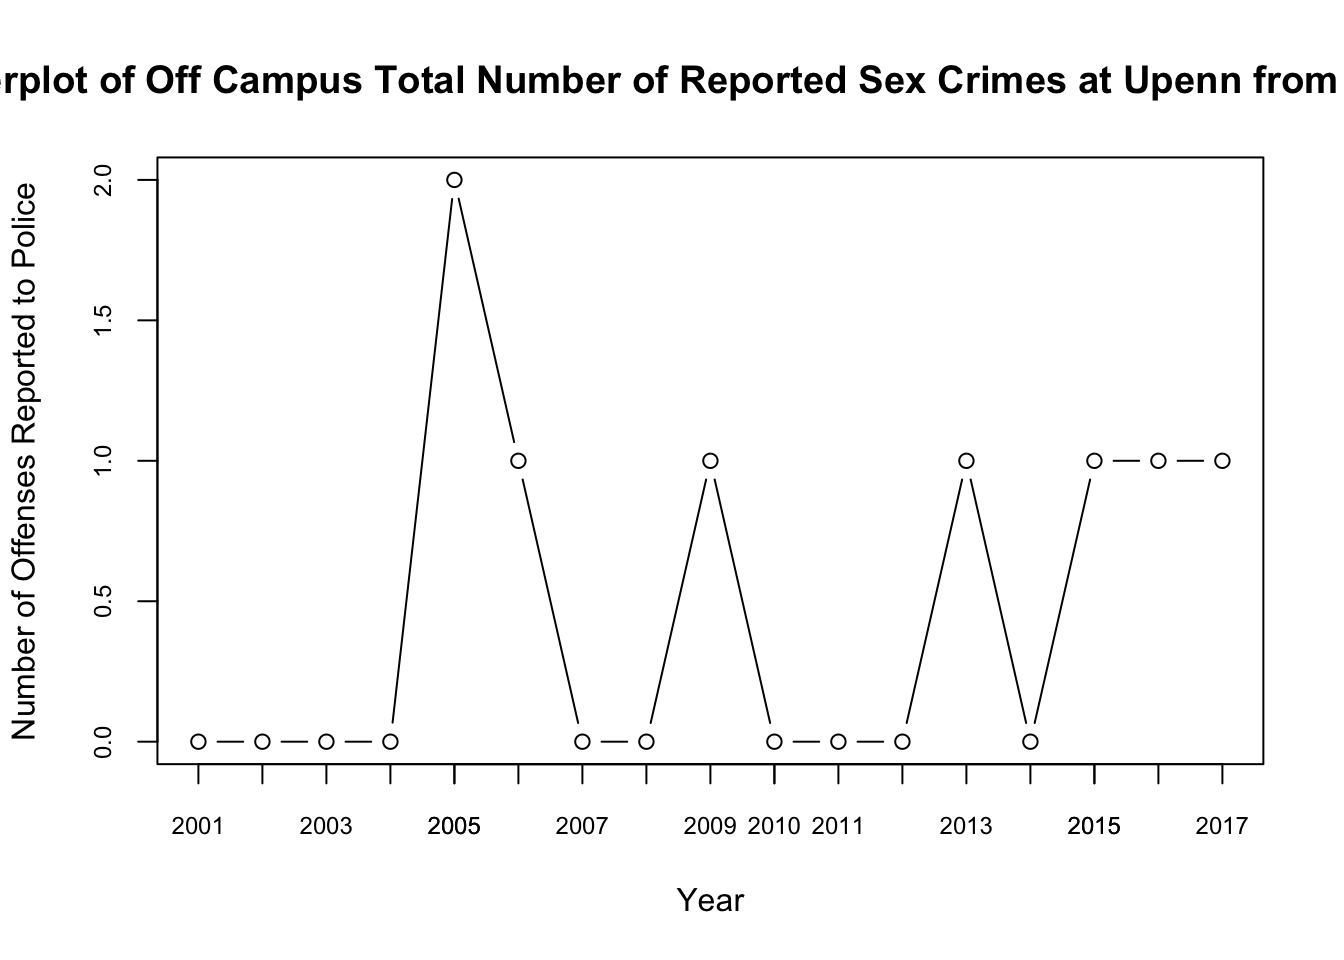
\includegraphics{Crim250FinalProj_files/figure-latex/unnamed-chunk-6-3.pdf}

\hypertarget{differences-in-different-crime-types}{%
\paragraph{2.8 DIFFERENCES IN DIFFERENT CRIME
TYPES}\label{differences-in-different-crime-types}}

\begin{figure}
\centering
\includegraphics{~/Desktop/testGitHub/SaraWhitR/ColumbiaBarGraph.png}
\caption{Differences In Different Crime Types}
\end{figure}

\begin{figure}
\centering
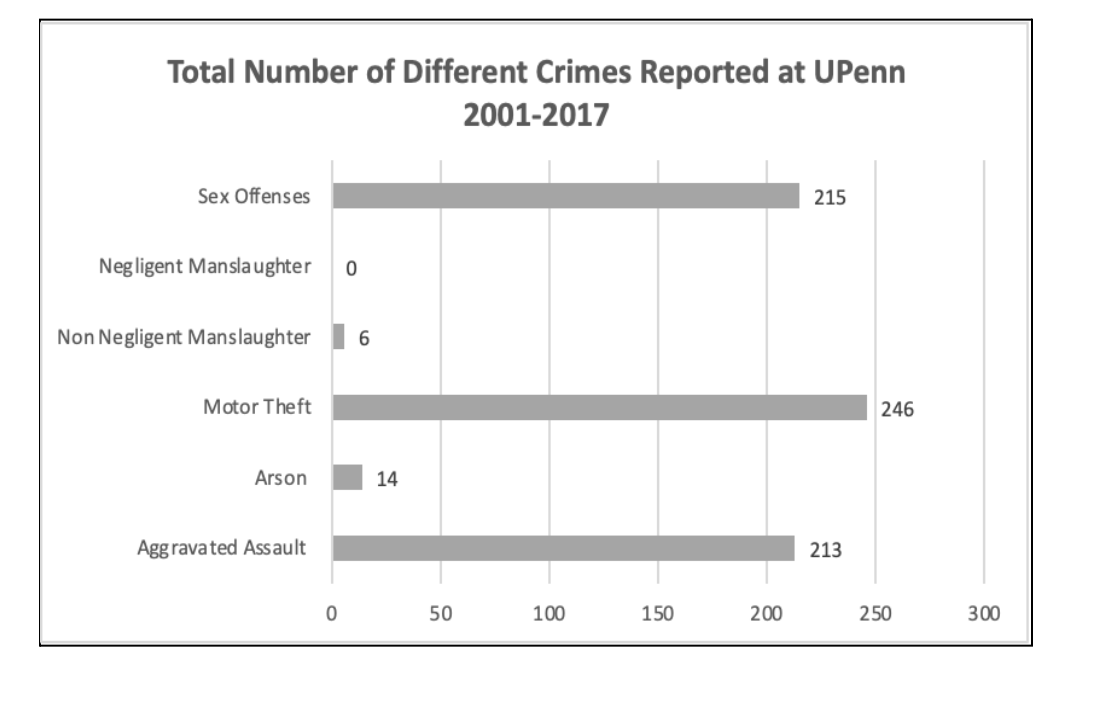
\includegraphics{~/Desktop/testGitHub/SaraWhitR/UpennBarGraph.png}
\caption{Differences In Different Crime Types}
\end{figure}

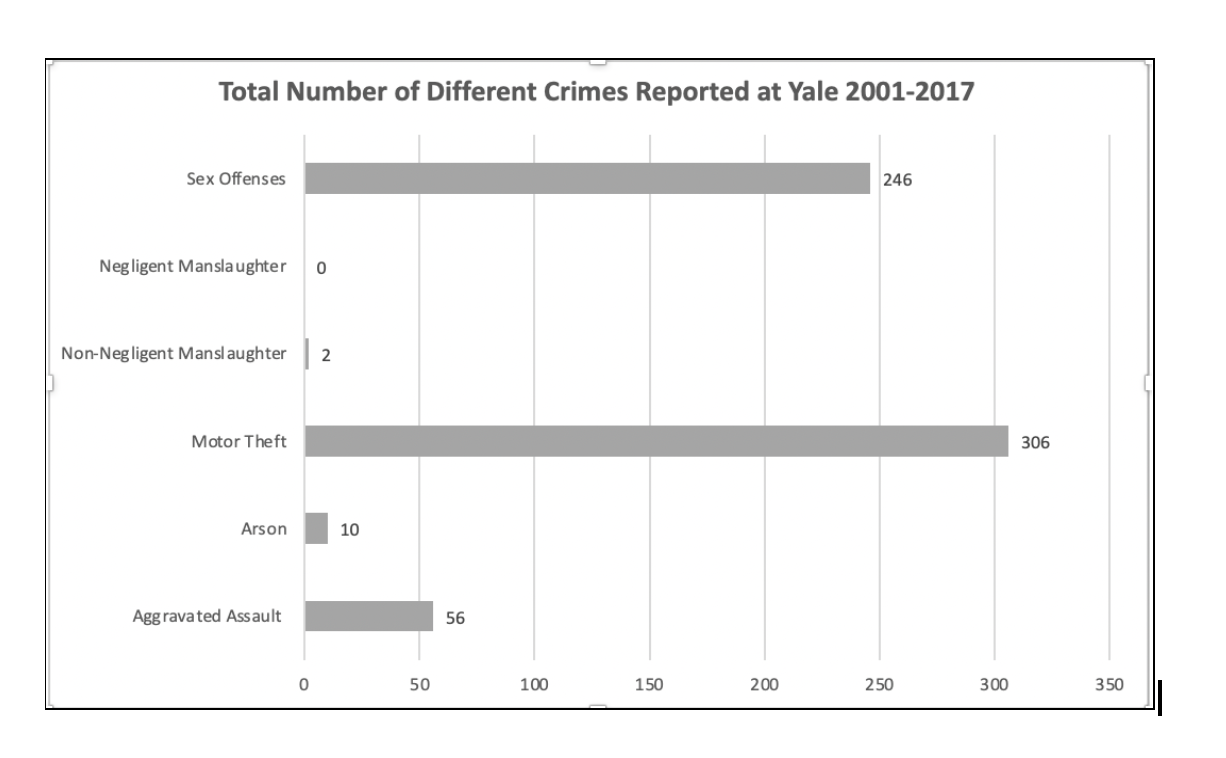
\includegraphics{~/Desktop/testGitHub/SaraWhitR/YaleBarGraph.png} \#
CAUSAL ANALYSIS

\hypertarget{causal-parameter-of-interest}{%
\paragraph{3.1 CAUSAL PARAMETER OF
INTEREST}\label{causal-parameter-of-interest}}

\begin{verbatim}
The causal parameters of interest are the size and funding of the police forces of the three Ivy League institutions: University of Pennsylvania, Yale University, and Columbia University. Additionally, we note the effect of Title IX guidelines on the sexual offense trends. While Columbia has 147 security officers rather than a private police force, Columbia benefits from the NYPD as they are located in the 26th precinct. Due to the size and power of the NYPD, Columbia’s total crime trend could be more reflective of the crime trends in the surrounding New York area. UPenn has a private police force of 121 sworn officers, which receives 27 million dollars of funding. UPenn’s negative crime trend could be a result of the robust size and funding of the police force, but without causal analysis and true experiments that include randomization, it is unclear whether this external factor has a relevant impact. Finally, on-campus sexual offense trends could be influenced by the causal parameter of Title IX guidelines and their implementation in university proceedings surrounding sexual offense cases. Title IX allows increased protections and assurance of investigation for on-campus students, which could possibly explain the high reporting rates for sexual offenses. Conversely, Title IX guidelines limit protections in off campus offenses noted in our discussion section.7 
It is important to note that these causal parameters can only be hypothesized as we do not have sufficient data to analyze whether they play an influential role in our EDA of the crime distributions of the three Ivy Leagues explored. 
\end{verbatim}

\hypertarget{proposed-causal-dag}{%
\paragraph{3.2 PROPOSED CAUSAL DAG}\label{proposed-causal-dag}}

The proposed causal DAG consists of two actions, the outcomes of the
actions, and the confounding variables that may impact both the actions
and the outcomes. In our case of understanding the crime distribution of
the Columbia, Yale, and UPenn, the actions that influence the crime
reporting rates are the strength and presence of the campus funded
police force and Title IX when regarding the reporting of sex offenses.
The expected outcomes of higher funding and strong on campus police
force would seemingly decrease total crime rates whereas decreased
funding and smaller police force would result in higher crime. Title
IX's on-campus guidelines would result in higher crime reporting of sex
offenses due to increased victim protection whereas their off campus
guidelines would result in decreased reporting. However, the confounding
variables that may impact both these actions and outcomes are reporting
bias, in that there may be failure to report by police offices as well
as failure to report by victim (sex assault), and the danger of the
location of the school.

\begin{figure}
\centering
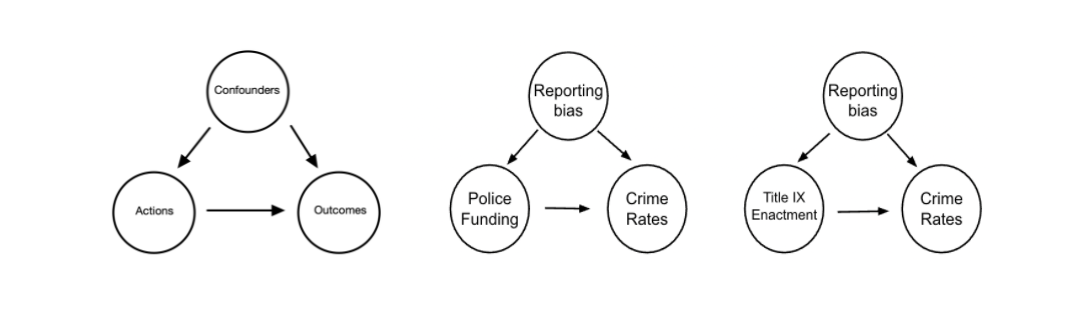
\includegraphics{~/Desktop/testGitHub/SaraWhitR/CausalDAG.png}
\caption{Causal DAG}
\end{figure}

\hypertarget{discussion}{%
\section{4. DISCUSSION}\label{discussion}}

We wanted to determine whether 1) There was a significant difference in
total crime rates and sexual offenses between three different urban, Ivy
League institutions, and 2) if police size and funding, and Title IX
guidelines influenced this relationship. Due to a lack of sufficient
data on which we could perform linear regression to explore the
correlation between these two actions (police funding and Title IX
guidelines), it is unclear whether they have an impact on the total
crime trends and sexual offense rates at any of the Ivy Leagues we
analyzed. However, overall, we found that the University of Pennsylvania
had the highest total number of reported crimes from 2001-2017, with a
total of 2069 crimes compared to Yale (1991) and Columbia (1589). It is
important to note that Columbia had two years of missing data, which
could change how its crime rates actually compare to the other
universities. Yale University had the highest number of reported sex
offenses (246) compared to Columbia University (196) and University of
Pennsylvania (216). We find this especially interesting because UPenn
has the highest crime rate, despite having the largest number of
on-campus sworn-in officers. Additionally, it is intriguing that Yale
University is located in the smallest city (population =130,250) of the
three schools analyzed, but still has the highest number of reported sex
offenses. Yale University also has the lowest police force funding (\$10
million), despite having the largest endowment (\$42.3 billion) of the
three Ivies.2,8,9 We also found that almost all sex offenses reported to
the respective campus police forces occurred on campus, rather than off
campus. It is possible that this is because off-campus sex offenses are
reported to the city police forces. In terms of Title IX providing
explanation for the stark difference between on campus and off campus
sexual offense trends, new Title IX guidelines do not require
universities to investigate events that occur off campus. Therefore,
there could ultimately be higher off campus sexual offense trends due to
lack of investigation by universities. Our results have some
limitations. The Columbia University data set was missing crime data for
2002 and 2004. The data sets that we used were subject to reporting bias
and missing data. Failure to report by police officers and failure to
report by victim, which is especially prevalent with sexual assault
cases, has an effect on the total number of crimes reported, as well as
the total number of sexual offenses reported. In addition, due to
limited data, we only used scatter and box plots to compare the crime
distribution and analyze the relationship between police force funding,
Title IX enactment, and crime distribution. The use of linear regression
would allow for strong analysis between these variables.

\hypertarget{appendix}{%
\section{5. Appendix}\label{appendix}}

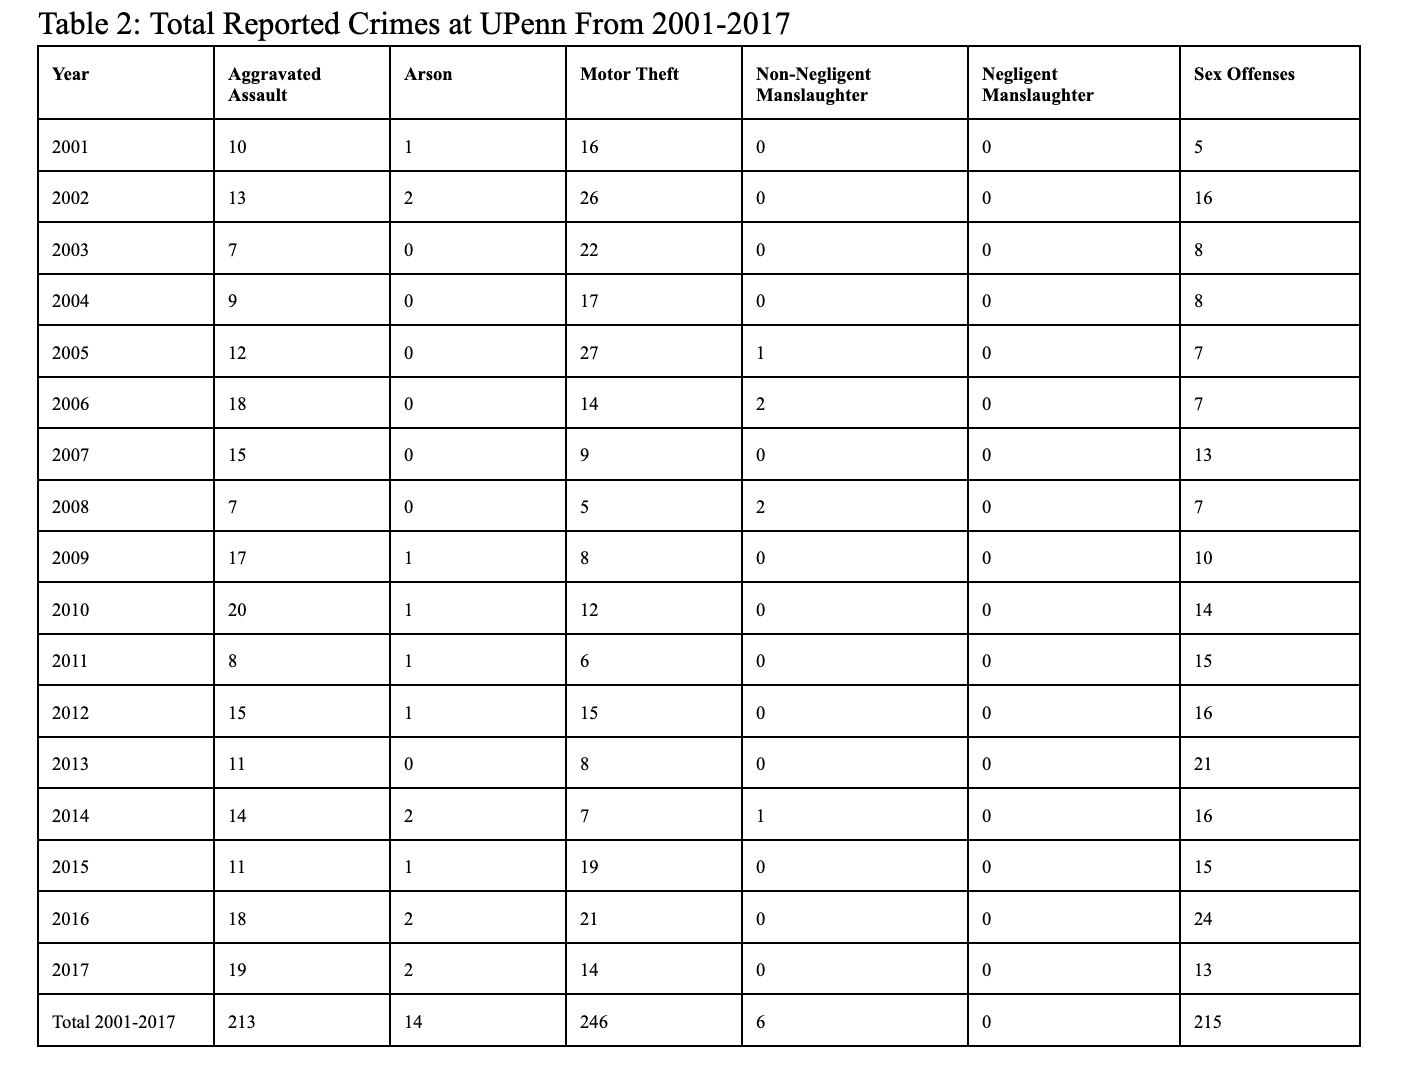
\includegraphics{~/Desktop/testGitHub/SaraWhitR/UpennAppendix.png}
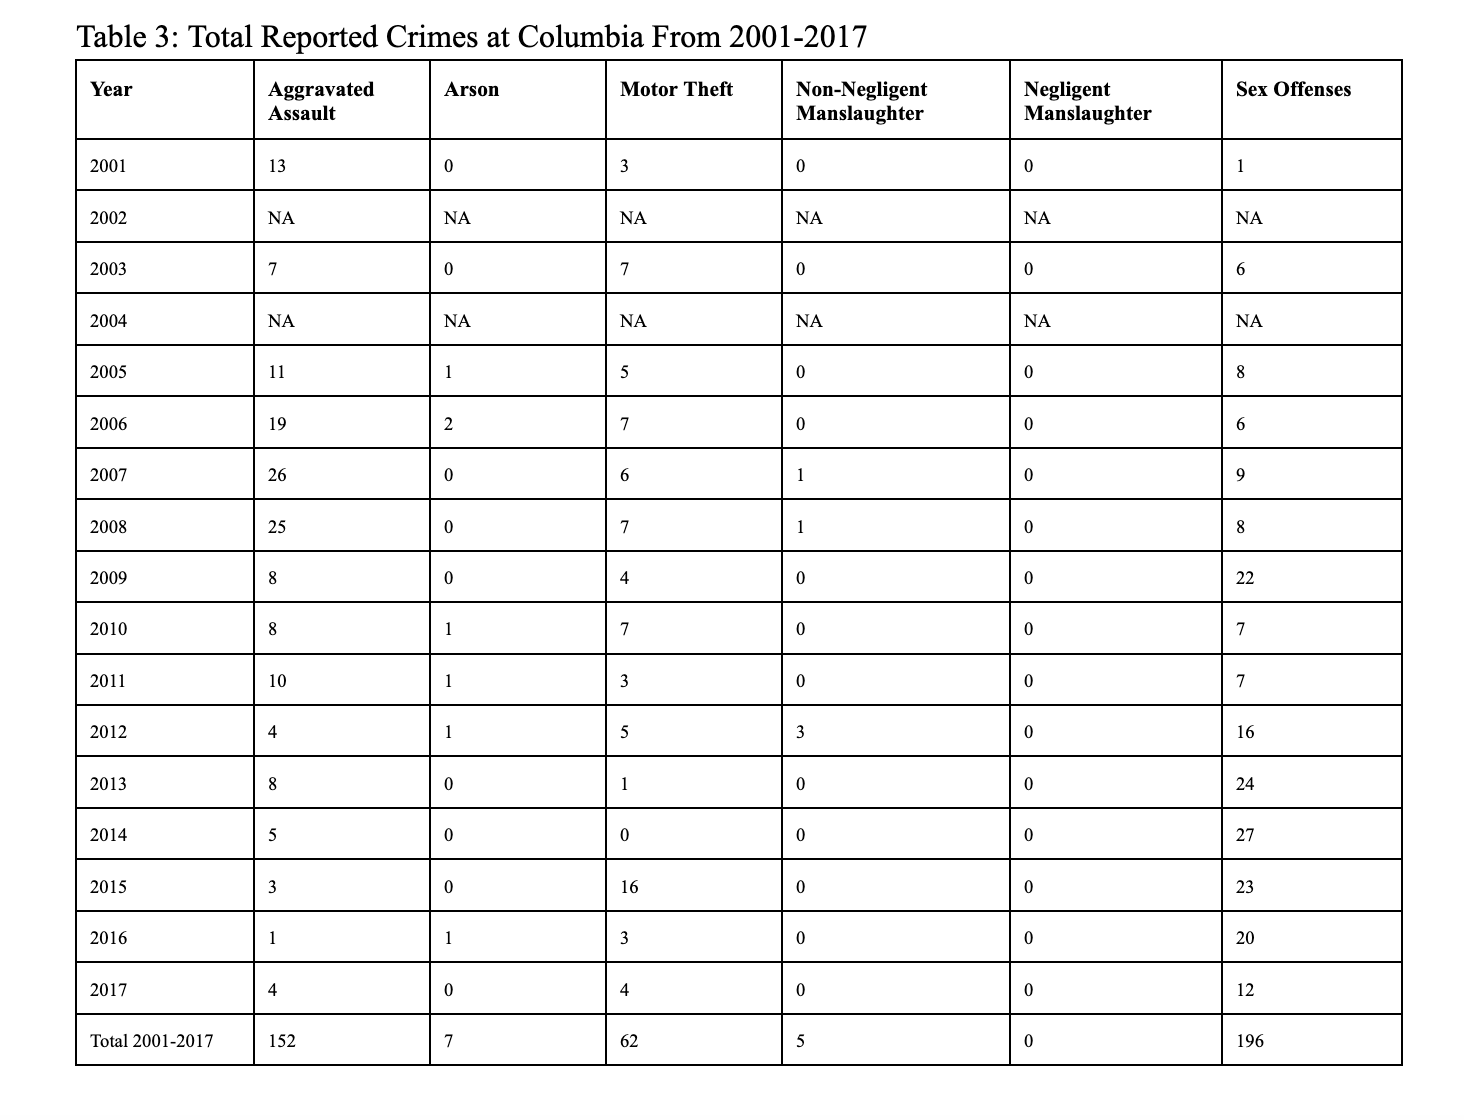
\includegraphics{~/Desktop/testGitHub/SaraWhitR/ColumbiaAppendix.png}

\begin{figure}
\centering
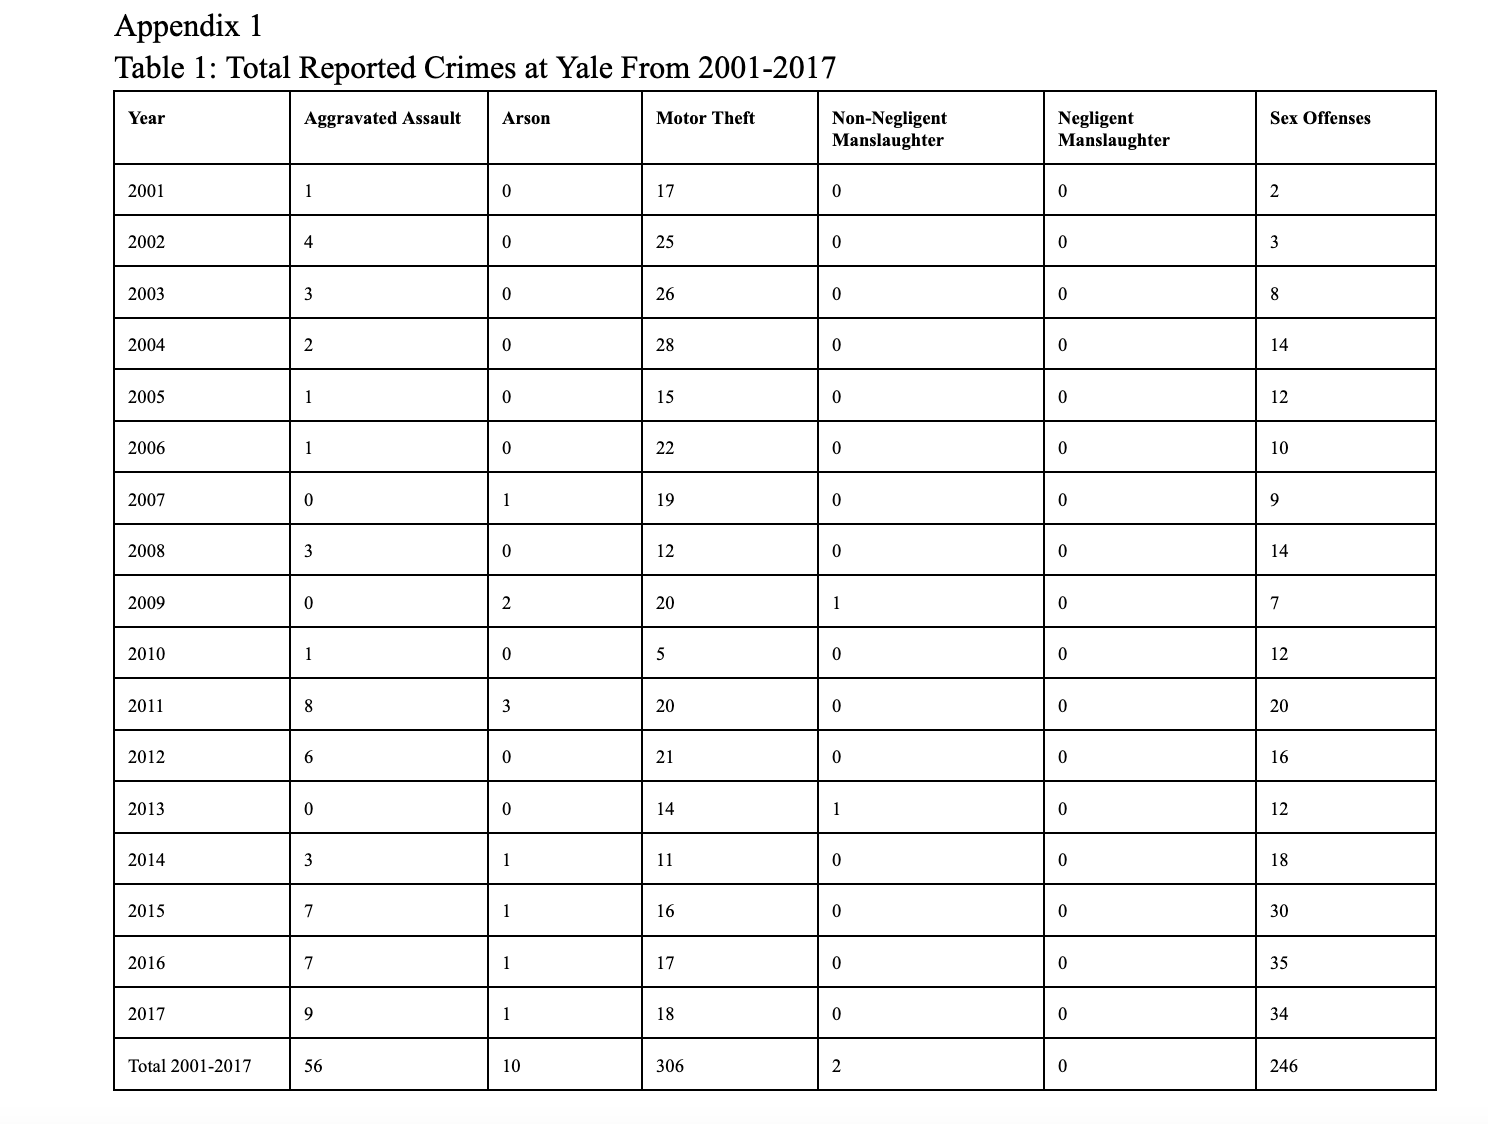
\includegraphics{~/Desktop/testGitHub/SaraWhitR/YaleAppendix.png}
\caption{Appendix 3}
\end{figure}

\hypertarget{sources}{%
\section{6 Sources}\label{sources}}

Kaplan, J. (n.d.). Crimes On University Campuses. Data \textbar{} Jacob
Kaplan. Retrieved December 7, 2021, from
\url{https://jacobdkaplan.com/data.html}. Bureau, U. S. C. (2021,
October 8). American Community survey 5-year data (2009-2019).
Census.gov. Retrieved December 7, 2021, from
\url{https://www.census.gov/data/developers/data-sets/acs-5year.html}.
Pennsylvania, U. of. (n.d.). About our division. Division of Public
Safety. Retrieved December 7, 2021, from
\url{https://www.publicsafety.upenn.edu/about/}. Yale University. (2020,
June). Yale Police Department. It's Your Yale. Retrieved December 7,
2021, from
\url{https://your.yale.edu/community/public-safety/yale-police-department}.
Heinzerling, K. (2017, October 8). With 120 officers, Penn has the
largest private police force in Pennsylvania. The Daily Pennsylvanian.
Retrieved December 7, 2021, from
\url{https://www.thedp.com/article/2017/10/with-120-officers-penn-has-the-largest-private-police-force-in-pennsylvania}.
26th precinct. 26 Precinct - NYPD. (n.d.). Retrieved December 7, 2021,
from
\url{https://www1.nyc.gov/site/nypd/bureaus/patrol/precincts/26th-precinct.page}.
Feldman, S. (2018, October 8). Yale and Title IX: A Complicated History
and an Unclear Future. The Politic. Retrieved December 7, 2021, from
\url{https://thepolitic.org/yale-and-title-ix-a-complicated-history-and-an-unclear-future/}.\\
Why: Black students for disarmament at Yale. bsdy. (n.d.). Retrieved
December 7, 2021, from \url{https://www.defundypd.com/why}. Yale
Investments Office. (n.d.). Retrieved December 07, 2021, from
\url{https://investments.yale.edu/}

\end{document}
